% No editar este archivo a menos que sepas que haces, para editar las secciones,
% ir a las diferentes secciones que estan divididas por archivos
\documentclass{edtclass}
\usepackage{graphicx}
\usepackage[justification=centering]{caption}
\usepackage[spanish]{babel}
\usepackage[utf8]{inputenc}
\usepackage{xcolor}
\usepackage{tabularx}

%\usepackage{showframe}


\begin{document}
% tables
\renewcommand{\tablename}{Tabla}
\renewcommand{\figurename}{Ilustración}

\begin{flushright}
    
\includegraphics[width=2cm]{imagenes/logo.png}  
  \end{flushright}
  
  \title{Este es un archivo template, debe cambiar este título}
  %\titlerunning{Short form of title} % if too long for running head
  
  \author{
    Autor Apellido Uno \authorlabel{1} \and 
    Autor Apellido Dos \authorlabel{2} %\and
  }
  %short form of author list (without footnote symbol) for running head; may be using "et al." 
  \authorrunning{A. Apellido Uno \and A. Apellido Dos}
  \institute{
    \authorlabel{1} Departamento de Ingeniería Civíl, Universidad, Direccion, Ciudad, País,
    \authoremail{1}{autorUno@apellidoUno.com}
    \and
    \authorlabel{2} Departamento de Ingeniería Civíl, Universidad, Direccion, Ciudad, País,
    \authoremail{2}{autorDos@apeliidoDos.com}
    %\and
  }
  
  % filled out by the editor: %%%%%%%%%%%%%%%%%%%%%%%%%%%%%%%%%%%%%%%
  \date{2020}{02/12/2020}{05/12/2020}{28/12/2020} % dates (received/revised/accepted)
  \identificacion{10.17815/CD.20XX.X} % doi 
  \volume{V}  % volume 
  \online{AX} % url 
  %%%%%%%%%%%%%%%%%%%%%%%%%%%%%%%%%%%%%%%%%%%%%%%%%%%%%%%%%%%%%%%%%%%
  
  \maketitle
   
  \keywords{Palabra clave 1 \and Palabra clave 2 \and Palabra clave 3}
  
  \begin{abstract}
    The objective of this work is to study the effect of design features such as door width, vestibule setback and vertical gap on passengers’ boarding and alighting time (BAT) at metro stations. Simulated experiments were performed at University College London’s Pedestrian Accessibility Movement Environment Laboratory (PAMELA). The mock-up included a hall or entrance to the train and a relevant portion of the platform in front of the doors. Different scenarios were tested based on existing stations. Results were compared to observations at Green Park Station of the London Underground (LU). Results from PAMELA showed that wider doors (1.80 m), larger vestibule setback (800 mm) and smaller vertical gap (50 mm) reduced the average boarding time. However, the average alighting time presented no significant differences due to other phenomenon such as congestion or formation of lines of flow at doors. The observation at LU presented a reduction of the BAT when a small vertical gap (170 mm) was presented. More experiments are needed at PAMELA to test the effect of the design features for different densities and types of passengers.
\end{abstract}

\clearpage
\section{Introduction}
\label{sec:intro}
El texto del artículo tiene interlineado sencillo; 12 puntos de tamaño de fuente; tipo de letra Times New Roman; las páginas están numeradas; se utiliza cursiva para las palabras en inglés en lugar de subrayado (excepto en las direcciones URL); y todas las ilustraciones, ecuaciones, figuras y tablas se encuentran enumeradas y colocadas en los lugares del texto apropiados, en vez de al final.
En la introducción se debe destacar el contexto/motivación del estudio, además del problema y los objetivos. Se puede incluir de forma opcional un texto con la estructura del artículo.

\section{Literature Review}
\label{sec:2}

At the PTI the BAT has been studied by different authors, showing the well-known linear relationship between the average time it takes for each passenger to board and alight, and the numbers of passenger boarding and alighting reported in the Highway Capacity Manual \cite{Ref7}. If the BAT is added to the time taken to open and close the doors, then the dwell time (td) is obtained. Based on this linear relationship Fernandez et al. \cite{Ref8} calibrated td for the case of Transantiago in Chile, in which the average boarding time was 40 percent higher than the alighting time in the metro system. 
Similarly, Tirachini \cite{Ref9} calibrated td using multiple regression models for the case of buses, in which td was influenced by the payment method, steps at doors, types of passengers (e.g. age) and the crowding situation. With respect to non-linear models, some authors have used the well-known LU Train Service Model to describe the BAT as part of the station stop time (SS) \cite{Ref10,Ref11}. The SS depends on the number of passengers boarding and alighting, the number of doors per car, the peak door/average door factor, the number of seats per car, the number of through passengers, and the door width factor \cite{Ref12,Ref13}.

Models have also been used to represent the boarding and alighting process. For example, according to Rudloff et al. \cite{Ref14} the social force model could predict the BAT. The authors found that the BAT decreased as the door width increased, reaching a minimum overall value of 24.93 secs for a door 185 cm wide. Other studies proposed a dwell time model based on smart card data \cite{Ref15} and using time-series based methods \cite{Ref16}. For Qi et al. \cite{Ref17}, the BAT is influenced by the perception and behaviour of passengers. The authors found that perception is influenced by the visual information captured by each passenger, the angle of movement, speed and density, whilst the behaviour depends on the distance, speed and time to get to the “target”. With respect to cellular automata models, each passenger boarding or alighting is represented within a square cell and their movement is recorded according to their negotiation and competition for positions/space. Zhang et al. \cite{Ref18} and Davidich et al. \cite{Ref19} studied the BAT, including the formation of lines of flow and the behaviour of passengers in waiting areas.

Different field studies have been carried out to support the different models in order to study the BAT at the PTI as reported by Li et al. \cite{Ref20}. In relation to the width of doors, Wiggenraad \cite{Ref21} found that wider doors decreased the BAT by 10 percent. The author studied five door widths in existing Dutch trains: 800mm, 900mm, 1100mm, 1300mm, and 1900mm. However, Harris et al. \cite{Ref22} reported that the relationship between door width and capacity is not linear, as the flow rate at doors is influenced by the available space on the platform and inside the train. In addition, Heinz \cite{Ref23} concluded that the BAT may be increased when the number of vertical steps is increased. The authors studied 18 different entrance designs at Swedish trains with level access, 2 steps, and 3 steps.

However, field studies are limited to the type of vehicles and stations existing at the time of study. It would be difficult to change the layout of the station or buy new vehicles to calibrate the models and to identify their effect on the BAT. In addition, it is impossible to control all the factors that influence the boarding and alighting for each observation. These factors are classified into four groups: people (e.g. density on the platform), physical aspects (e.g. platform width), information (e.g. on-board displays), and environmental influences (e.g. weather) \cite{Ref24}.

To solve this, various laboratory experiments have been done at PAMELA. These experiments have been very useful in singling out the influence of a particular variable because only one particular variable could be changed while keeping the other variables the same. One of the first laboratory studies done by Fernandez et al. \cite{Ref25} showed that the BAT is influenced by the door widths (0.80 m and 1.60 m) and the different fare collection systems. The authors simulated the boarding and alighting in a bus and they found that wider doors (1.60 m) reduced the alighting time by 40 percent, while the boarding time was reduced by up to 45 percent by payment being made outside the vehicle (using a ticket vending machine on the platform).  That study was followed by an experiment done by Seriani and Fernandez \cite{Ref26} to simulate the boarding and alighting in a train at the Human Dynamics Laboratory (HDL) in Universidad de los Andes, in which the BAT was influenced by the vertical handrails, waiting areas on the platform, and the use of one-way doors. Recent experiments performed by De Ana Rodriguez et al. \cite{Ref27} showed that the use of platform edge doors (PEDs) has no relevant impact on the BAT, however, passengers change their behaviour by queuing at the side of the doors rather than waiting in front of them. Following the study of PEDs, Seriani et al. \cite{Ref28} explored the Level of Interaction (LOI) at PAMELA, where passengers reached a high LOI near the doors, which decreased as the distance from the doors increased. This study was expanded by Seriani and Fujiyama \cite{Ref29} to calculate the space used by each passenger alighting at PAMELA when PEDs were installed.

In relation to steps, Holloway et al. \cite{Ref30} simulated laboratory experiments at PAMELA in which the use of steps was considered an obstacle for passengers boarding and alighting. In this case the authors simulated 60 passengers boarding and alighting with one single door and three different steps: 20 mm (zero step), 350 mm (2 steps), and 510 mm (3 steps). The authors found that boarding passengers spent more time (4.13 seconds on average) than those who were alighting (3.68 seconds on average), and 40 percent of the total passengers found it difficult to use steps when they were boarding and alighting. In the same line of research, experiments at TU Delft done by Daamen et al. \cite{Ref31} reported that steps can influence the capacity of doors. In this experiment the authors tested four steps: 50 mm (zero step), 200 mm (1 step), 400 mm (2 steps), and 600 mm (3 steps); and three horizontal gaps: 50 mm, 150 mm, and 300 mm. The authors found that the capacity of the doors decreased from 0.91 passengers per second (pps) to 0.81 pps when changing the step from 50 mm to 400 mm. In this case the horizontal gap was 50 mm and the door width 80 cm. However, the authors also found that for a horizontal gap of 300 mm and the same door width (80 cm), the capacity increased from 0.85 pps to 0.88 pps when changing the step from 50 mm to 200 mm.

It is generally thought that to improve accessibility at the PTI the difference in height (vertical) and distance (horizontal) between the vehicle and the platform should be reduced to their minimum. Some studies performed by Atkins \cite{Ref32} recommend that the sum between the horizontal and the vertical gap should not exceed 300 mm, and that an optimum value for design would be 200 mm. If the vertical gap is more than 50 mm and the horizontal gap more than 75 mm, then a boarding device is needed for passengers with restricted mobility (e.g. wheelchairs) [6]. When these values are not in place along the complete platform, Tyler et al. \cite{Ref33} propose to build platform humps, by which only a part of the platform is raised to be level with the vehicle. The authors tested different slopes and cross-fall gradients at PAMELA, in case the vehicle should not stop directly in front of the ramp.

Although the vertical gap could be considered as a negative aspect in providing accessibility, in some cases it could improve the boarding and alighting process. Recently laboratory studies at HDL showed that a small vertical gap can decrease the BAT. Fernandez et al. \cite{Ref34} found that for a door width of 1.65 m the best vertical gap may be 150 mm, allowing an alighting flow of 1.6 passengers per second. In this experiment only alighting was simulated, considering three scenarios of vertical gap: 0 mm, 150 mm, and 300 mm. From another study at PAMELA, Fujiyama et al. \cite{Ref35} simulated bidirectional flows (i.e. boarding and alighting) and suggested that the PTI should be designed with a vertical gap of 50 mm, allowing a maximum flow of 1.42 passengers per second. From these results a model was proposed by Karekla et al. \cite{Ref36} to predict the dwell time was proposed, in which a small vertical gap reduced the dwell time by 8 percent. 

Other authors have studied bottlenecks to simulate the movement of pedestrians through a single door by laboratory experiments. In the case of Kretz et al. \cite{Ref37} examined different door width (40, 50, 60, 70, 80, 90, 100, 120, 140 and 160 cm) and found that if the bottleneck is 90 cm or above then two or more participants were able to pass. The author also reported that a competitive scenario presented smaller evacuation time compared to the non-competitive scenario. Hoogendoorn and Daamen \cite{Ref38} studied the effect of the width of the bottleneck and the wall surface. The authors found that pedestrian followed the pedestrian directly in front and when the distance between them is about 45 cm then the zipper effect is reached (e.g. pedestrian are overlapped forming two lines of flow). This is caused because pedestrian need more space to move forward than to move in lateral way. However, Seyfried et al. \cite{Ref39} also used unidirectional flow in a bottleneck cantered of a corridor (similar to \cite{Ref37}) and found that the density in front of the bottleneck has a major impact on the flow, in which the zipper effect (overlapped pedestrians) began to act when the door reached 70 cm width. Recently, Adrian et al. \cite{Ref40} did 2 runs per group and studied the width of the bottleneck for different scenarios: 1.2 m, 2.3 m, 3.4 m, 4.5 m, and 5.6 m. The authors reported that the demand level affects the behaviour of pedestrians in the bottleneck (e.g. pushing).

In spite of different research having being carried out to study the layouts of vehicles and stations, more detailed research was needed to identify the effect of design features  on the BAT. The observations made from the results of the experiments presented in this paper would fill gaps and reconfirm important points in relation to existing studies. In particular, it could be interesting to compare the results from laboratory experiments at PAMELA with real data observed at LU stations.

\section{Métodos}
\label{sec:3}

El texto del artículo tiene interlineado sencillo; 12 puntos de tamaño de fuente; tipo de letra Times New Roman; las páginas están numeradas; se utiliza cursiva para las palabras en inglés en lugar de subrayado (excepto en las direcciones URL); y todas las ilustraciones, ecuaciones, figuras y tablas se encuentran enumeradas y colocadas en los lugares del texto apropiados, en vez de al final.
En esta sección se debe explicar:
\begin{itemize}
    \item La metodología, la toma de datos, uso de encuestas, modelos, etc. 
    \item También se puede incluir restricciones en el método usado. 
\end{itemize}


Además, se debe definir las variables a utilizar, los escenarios a estudiar (ver Tabla \ref{tab1}), y la forma de comparar dichos escenarios, entre otros.

\begin{table}
  \centering
  \begin{tabular}{cl}
    \toprule
      Brecha vertical (mm) & Experimentos\\
    \midrule
        0 & Caso Base             \\ 
        50 & Parada con andén     \\
        100 & No existente        \\
        150 & Parada normal       \\
        200 & No existente        \\
    \bottomrule
  \end{tabular}
  \caption{Ejemplo de escenarios a utilizar en este estudio}
  \label{tab1} % unique label

\end{table}

\section{Resultados}
\label{sec:4}

\subsection{Sección 1 de Resultados}
\label{sec:4.1}

El texto del artículo tiene interlineado sencillo; 12 puntos de tamaño de fuente; tipo de letra Times New Roman; las páginas están numeradas; se utiliza cursiva para las palabras en inglés en lugar de subrayado (excepto en las direcciones URL); y todas las ilustraciones, ecuaciones, figuras y tablas se encuentran enumeradas y colocadas en los lugares del texto apropiados, en vez de al final.
Además, se pueden incluir secciones para agrupar resultados, por ejemplo, según escenarios o método a usar.
Los resultados se pueden ver en tablas o ilustraciones, las cuales pueden complementar la explicación del texto (ver \reffigura{fig1}{Ilustración 1}).

\begin{figure}[h]
    \centering
    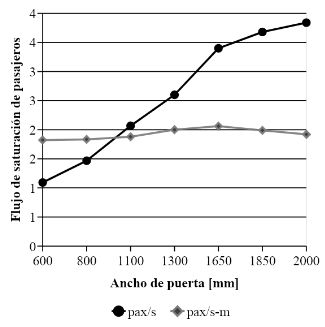
\includegraphics[width=0.5\textwidth]{imagenes/fig1.png}
    \caption{Flujo de saturación de pasajeros en función del ancho de puertas}\label{fig1}
\end{figure}

\section{Discussion}
\label{sec:5}
El texto del artículo tiene interlineado sencillo; 12 puntos de tamaño de fuente; tipo de letra Times New Roman; las páginas están numeradas; se utiliza cursiva para las palabras en inglés en lugar de subrayado (excepto en las direcciones URL); y todas las ilustraciones, ecuaciones, figuras y tablas se encuentran enumeradas y colocadas en los lugares del texto apropiados, en vez de al final.
En esta sección se puede hacer comentarios de cierre del estudio, además de discusiones y futuras investigación. También se puede incluir en el texto un resumen destacando los resultados relevantes.
\\
Ejemplo para las citas \cite{einstein} o \cite{knuthwebsite,latexcompanion}
Ejemplo para referenciar ecuación 
\begin{equation}
    \label{ecuacion:circulo}
    a^2 + b^2 = c^2
\end{equation}
Ejemplo para las referencias 
\begin{itemize}
    \item \refseccion{sec:2}
    \item \reftabla{tab1}
    \item \reffigura{fig1}
    \item \refecuacion{ecuacion:circulo}
\end{itemize}
\begin{agradecimientos}
  Los autores pueden incluir esta sección donde se agradece, por ejemplo, el financiamiento de los proyectos, memoristas, o a quienes participaron de los experimentos/encuestas, etc. 
\end{agradecimientos}
\bibliography{bibliography}
\bibliographystyle{apalike}


\end{document}